\chapter{Transformações Lineares}
Neste capítulo, iremos tratar sobre um tipo especial de função ou aplicação, onde, segundo \cite{steinbruch1987}, o domínio e o contradomínio são espaços vetoriais reais. Assim, tanto a variável independente como a variável dependente são vetores, razão pela qual essas funções são chamadas vetoriais.

Nosso estudo das funções vetoriais lineares em questão, será focado, nas transformações lineares.

\noindent\textbf{Definição 04:} Sejam $\mathbf{V}$ e $\mathbf{W}$ dois espaços vetoriais. Uma transformação linear (aplicação linear) é uma função de $\mathbf{V}$ em $\mathbf{W}$, tal que, $\mathbf{T}: \mathbf{V} \rightarrow \mathbf{W}$, que satisfaz as seguintes condições:

\begin{enumerate}
	\item Para quaisquer $\mathbf{u}$ e $\mathbf{v}$ em $\mathbf{V}$, $\mathbf{T}(\mathbf{u} + \mathbf{v}) = \mathbf{T}(u) + \mathbf{T}(v)$.
	\item Para quaisquer $k \in \mathbb{R}$ e $\mathbf{v} \in \mathbf{V}$, $F(k\mathbf{v}) = k\mathbf{F}(\mathbf{v})$.
\end{enumerate}	

No caso especial em que $\mathbf{V} = \mathbf{W}$, a transformação linear é denominada \textbf{operador linear} do espaço vetorial $\mathbf{V}$ \cite{anton2010elementary}.

\noindent\centerline{Válido em: $\forall \mathbf{v}, \mathbf{v} \in \mathbf{V}$ e $\forall k \in \mathbb{R}$. }

Para se dizer que $\mathbf{T}$ é uma transformação linear do espaço vetorial $\mathbf{V}$ no espaço vetorial $\mathbf{W}$, será denotado por $\mathbf{T}:\mathbf{V}\longrightarrow\mathbf{W}$, onde $\mathbf{T}$ é a função, cada vetor $\mathbf{v} \in \mathbf{V}$ tem uma só imagem $\mathbf{w} \in \mathbf{W}$, indicado por $\mathbf{w} = \mathbf{T}(\mathbf{v})$.

Tomemos por dois conjuntos de vetores, $\mathbf{V} = \mathbb{R}^2$ e $\mathbf{W} = \mathbb{R}^3$.

Uma transformação de $\mathbf{T}:\mathbb{R}^2\longrightarrow\ \mathbb{R}^3$ associa vetores $\mathbf{v} = (x, y) \in \mathbb{R}^2$ com vetores $\mathbf{w} = (x, y, z) \in \mathbb{R}^3$

\noindent\textbf{Exemplo 11:} Declarado esta transformação linear $\mathbf{T}(x, y) = (x, y, x + y)$. Iremos selecionar alguns vetores em $\mathbb{R}^2$ e calcular suas imagens sob a transformação $\mathbf{T}$. Por exemplo, os vetores $(1, 0)$ e $(0, 1)$. Para $(1, 0)$, temos: 

\begin{equation}
	\mathbf{T}(1, 0) = (1, 0, 1 +0) = (1, 0, 1)
\end{equation}

\noindent e para $(0, 1)$, temos:

\begin{equation}
\mathbf{T}(0, 1) = (0, 1, 0 + 1) = (0, 1, 1)
\end{equation}

Segue a imagem em $\mathbb{R}^3$:

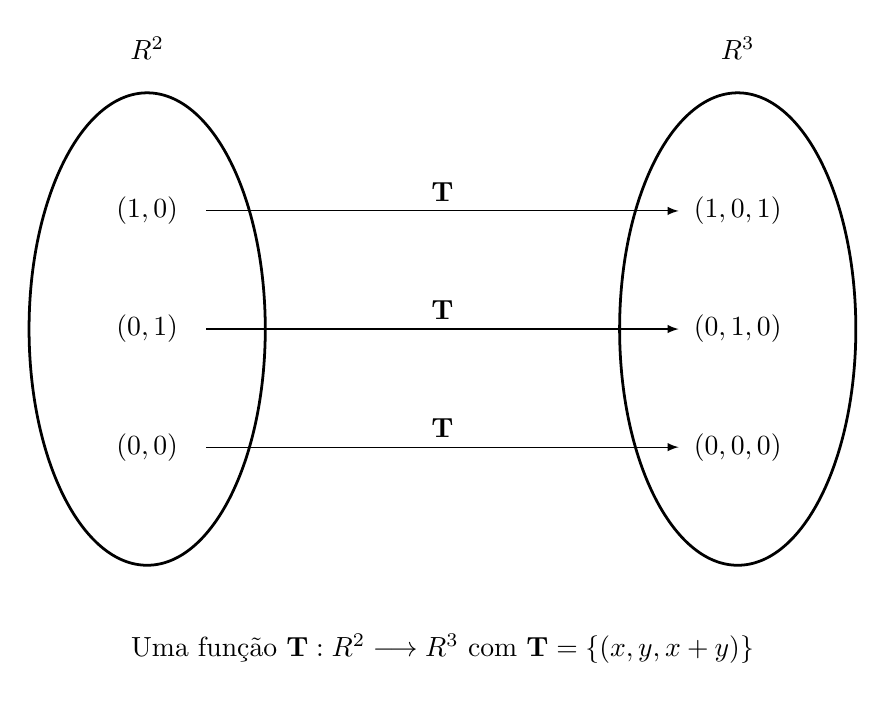
\begin{tikzpicture}[scale=1.5]
	\centering
	% Set A
	\draw[line width=1pt] (0,0) ellipse (1cm and 2cm);
	\node[above] at (0,2.2) (A) {$\mathbb{R}^2$};
	\node[centered] at (0,1) {$(1,0)$};
	\node[centered] at (0,0) {$(0,1)$};
	\node[centered] at (0,-1) {$(0,0)$};
	% Set B
	\draw[line width=1pt] (5,0) ellipse (1cm and 2cm);
	\node[above] at (5,2.2) (B) {$\mathbb{R}^3$};
	\node[centered] at (5,1) {$(1,0,1)$}; 
	\node[centered] at (5,0) {$(0,1,0)$};
	\node[centered] at (5,-1) {$(0,0,0)$};
	
	% Relations
	\draw[-latex, black] (0.5,1) -- node[midway, above] {$\mathbf{T}$} (4.5,1);
	\draw[-latex, black] (0.5, 0) -- node[midway, above] {$\mathbf{T}$} (4.5, 0);
	\draw[-latex, black] (0.5, -1) -- node[midway, above] {$\mathbf{T}$} (4.5, -1);
	
	% Label
	\node[below] at (2.5,-2.5) {Uma função $\mathbf{T}: \mathbb{R}^2 \longrightarrow \mathbb{R}^3$ com $\mathbf{T}=\{(x, y, x + y)\}$};
\end{tikzpicture}

\noindent\textbf{Exemplo 12:} Se tomarmos um vetor arbitrário e fazemos uma transformação linear idêntica, ou seja, $1\alpha$ = $\alpha$, é uma transformação linear de $\mathbf{V}$ em $\mathbf{V}$. A transformação é definida por $0\alpha = 0$, é também uma transformação linear de $\mathbf{V}$ em $\mathbf{V}$ \cite{hoffman1979}.

De acordo com o exemplo acima, percebe-se, que será uma função onde o gráfico passa a reta pela origem se supormos uma função afim, $\mathbb{R}^1$ em $\mathbb{R}^1$. Uma transformação linear mantém combinações lineares $W = [\mathbf{v}_1, \ldots, \mathbf{v}_n]$ são vetores que pertencem a $\mathbf{V}$ e possui seus escalares $c_1, \ldots, c_n$, então:

\begin{equation}
\mathbf{T}(c_1\mathbf{v}_1, \ldots, c_n\mathbf{v}_n) = \mathbf{T}(c_1\mathbf{v}_1 + c_2\mathbf{v}_2) = c_1(\mathbf{T}\mathbf{v}_1) + c_2(\mathbf{T}\mathbf{v}_2)
\end{equation}

\noindent\textbf{Exemplo 13:} Tomemos um caso que desejamos dobrar nosso espaço vetorial, dado um vetor $\mathbf{V} = (2, 2); \mathbf{V} \in \mathbb{R}^2$, a transformação linear será dada por, $\mathbf{T}(x, y) = (2x, 2y) \in \mathbb{R}^2$. Nosso domínio e contradomínio está em $\mathbb{R}^2$, portanto o resultado será por $\mathbf{W} = (2 \times 2, 2 \times 2) \therefore \mathbf{W} = (4, 4)$

\begin{figure}[H]
	\centering
	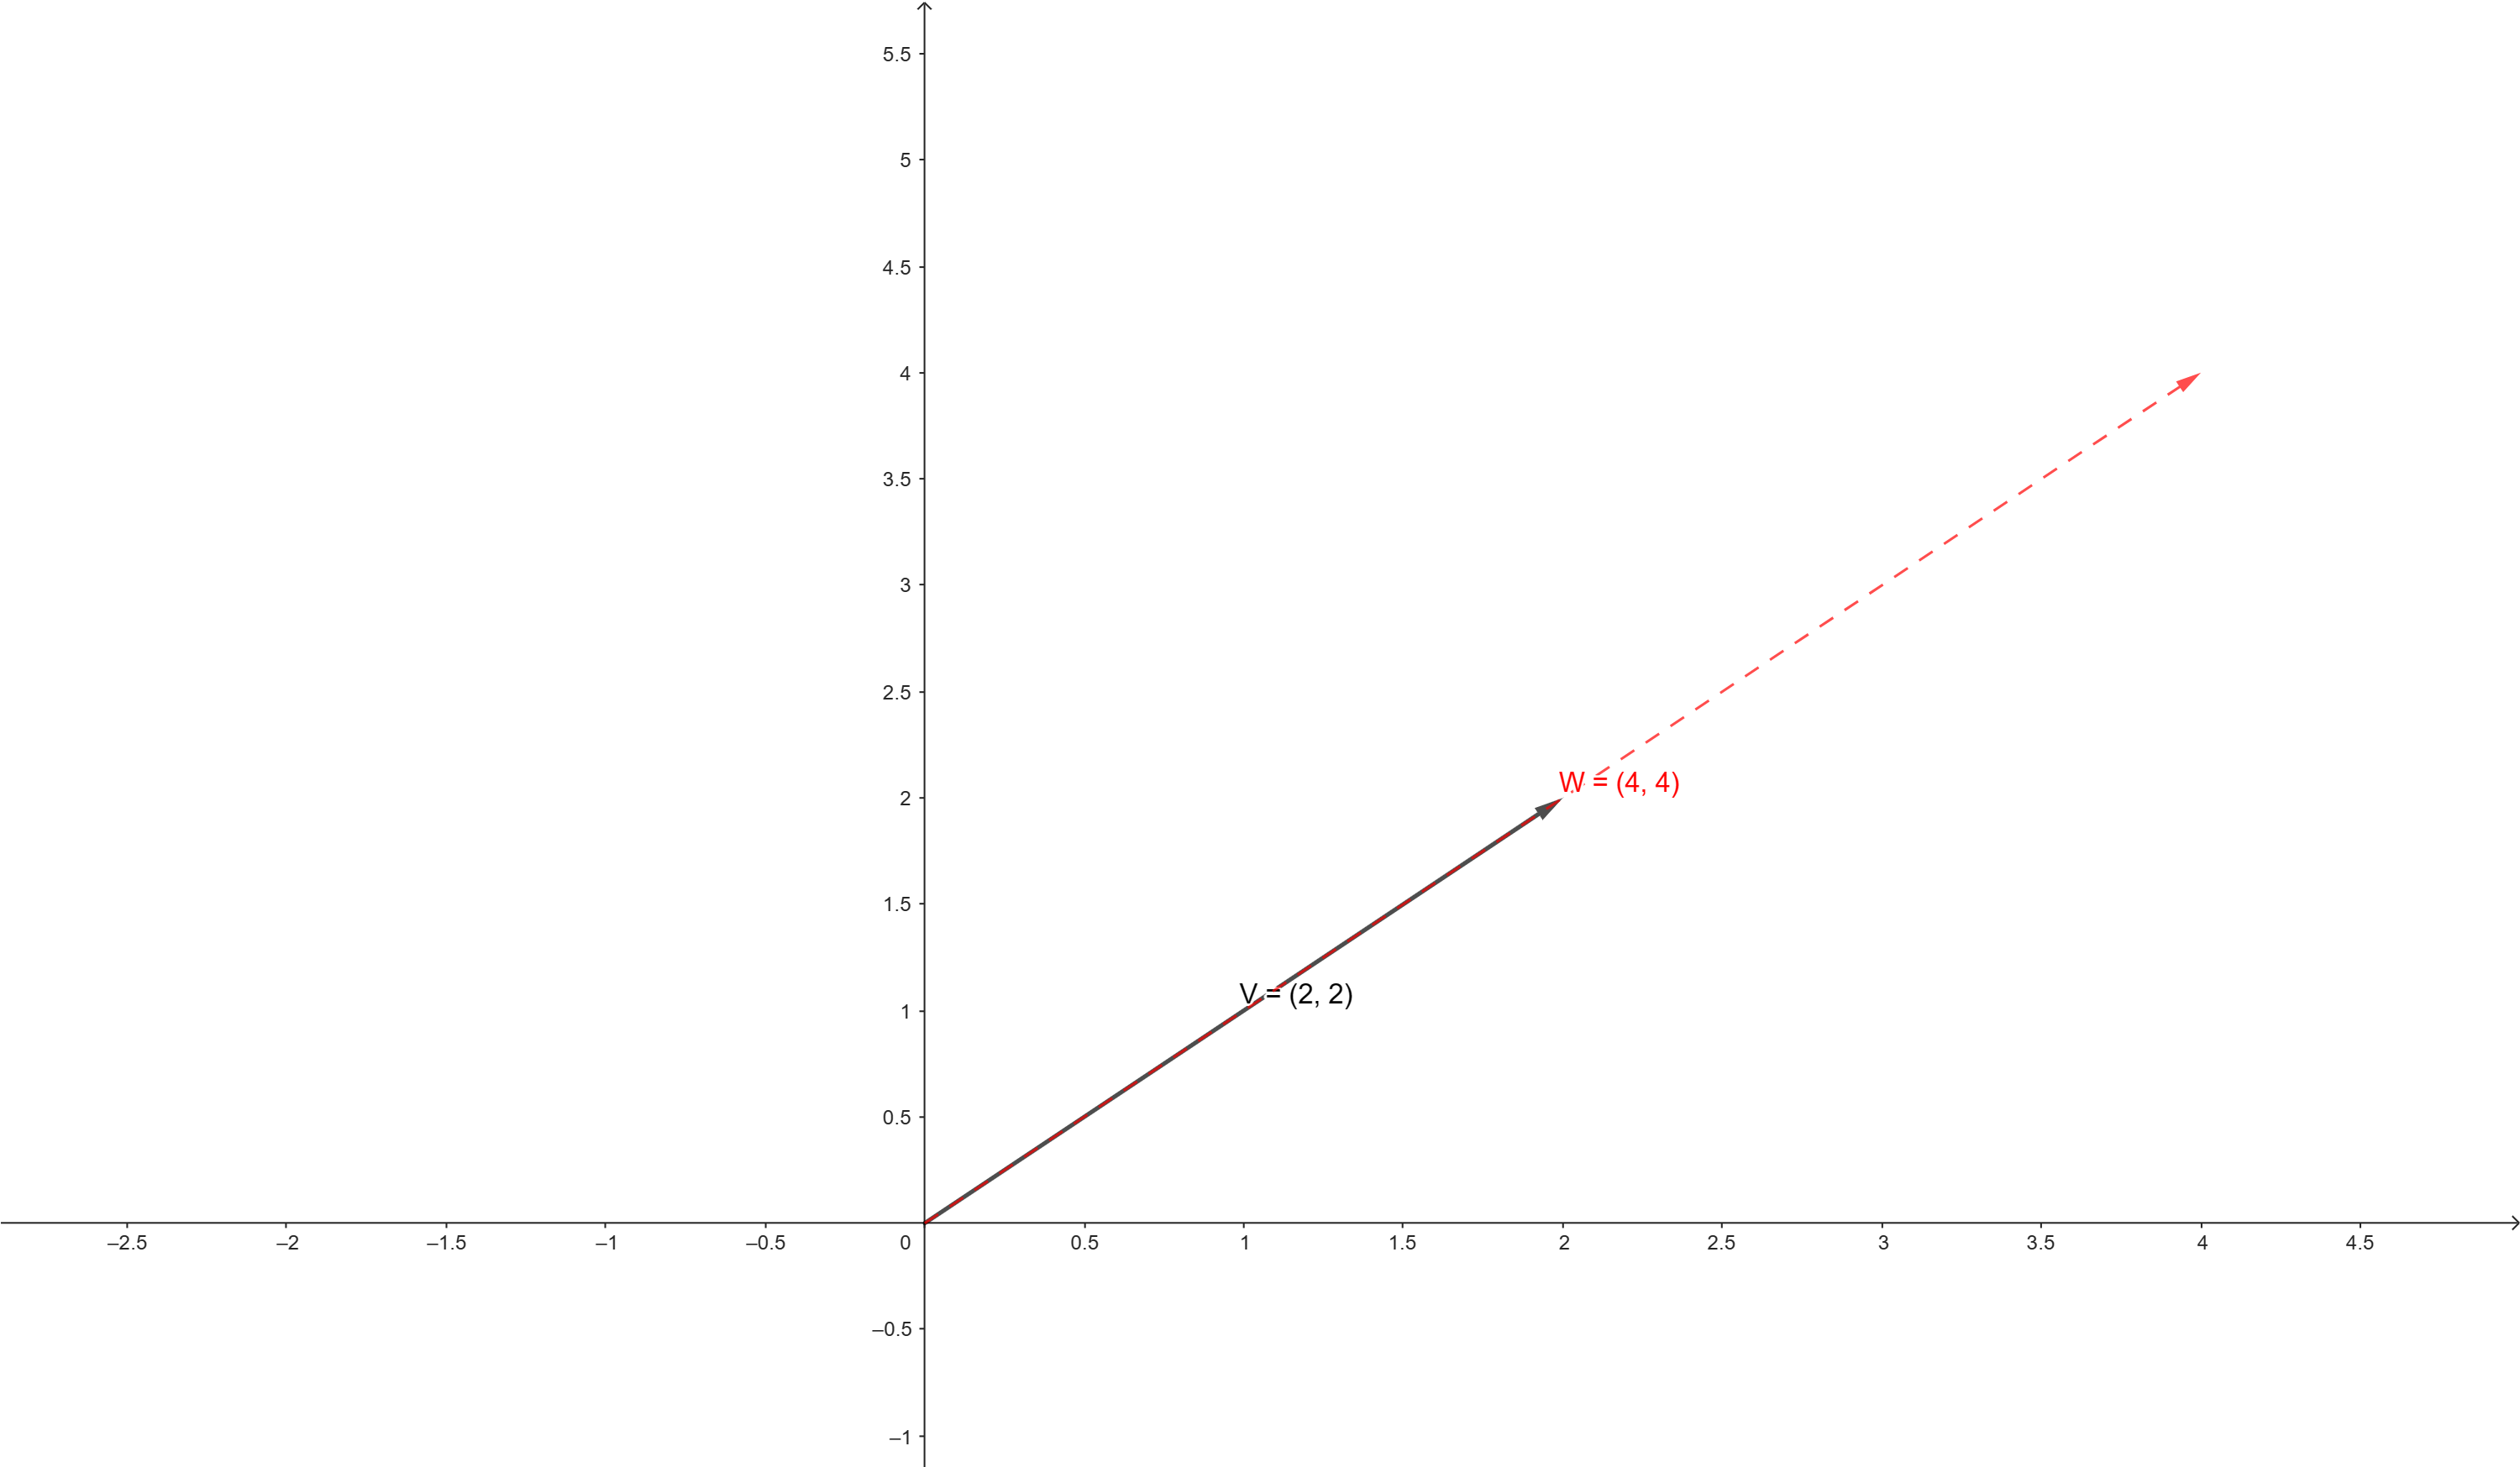
\includegraphics[scale=1.30]{t_exemplo13.png}
	\caption{Transformação linear dobro de um vetor.}
\end{figure}

Para uma matriz de transformação linear $\mathbf{T}$ de $\mathbf{V}$ em si mesma, existe uma matriz única $\mathbf{A}$ de dimensão $ n \times n$ que representa $\mathbf{T}$. Essa matriz é definida pela seguinte propriedade:

\centerline{$\mathbf{T}(\mathbf{v} = \mathbf{A}\mathbf{v})$}

\noindent para todo vetor $\mathbf{v}$ em $\mathbf{V}$. A matriz $\mathbf{A}$ é chamada de matriz de transformação de $\mathbf{T}$.

% Primeira aplicação citada da transformação
Consideremos agora no segmento da transformação linear e no campo da geometria o uso de operações como rotações, reflexões e projeções. Tomemos o espaço vetorial bidimensional $\mathbb{R}^2$ com base canônica $\mathbf{e}_1 = (1, 0)$ e $\mathbf{e}_2 = (0, 1)$. A rotação de 90 graus no sentido anti-horário pode ser representada pela seguinte matriz de transformação:

\centerline{$\mathbf{R} = [[0, 1], [-1, 0]]$}

A matriz $\mathbf{R}$ chamada de matriz de rotação, possui algumas propriedades:

\begin{enumerate}
	\item \textbf{Ortogonalidade:} A matriz $\mathbf{R}$ é ortogonal, ou seja sua transporta é inversa:
	
	\centerline{$\mathbf{R}^T = \mathbf{R}^{-1}$}
	\item \textbf{Determinante:} O determinante da matriz $\mathbf{R}$ é igual a $-1$.
	
	\centerline{$\det(\mathbf{R}) = -1$}
\end{enumerate}

Ao rotacionar um vetor $\mathbf{v} = (x, y)$ em 90 graus  no sentido anti-horário, basta aplicar a matriz de rotação em $\mathbf{v}$.

\begin{equation}
\mathbf{v}' = \mathbf{R} \times \mathbf{v} = [[-1, 0], [0, -1]] \times [x, y] = [y, -x]
\end{equation}

No caso em questão, o operador de rotação de um angulo qualquer como $\theta$ em torno e origem em $\mathbb{R}^2$, tratando-se o operador $\mathbf{R}: \mathbb{R}^2 \longrightarrow \mathbb{R}^2$, resulta em $\mathbf{R}(u + v) = \mathbf{R}(u) + \mathbf{R}(v)$.

\begin{figure}[H]
	\centering
	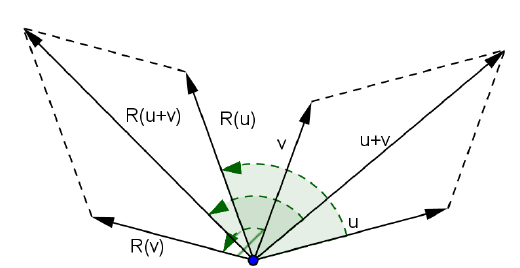
\includegraphics[scale=0.90]{t_rotacao.png}
	\caption{Transformada de rotação de um vetor \cite{nogueira2013}.}
\end{figure}

\section{Núcleo de uma Transformação Linear}
Em transformações lineares. O núcleo, também chamado de espaço nulo de uma transformação linear $\mathbf{T}$, denotado por  $\mathbf{N}(\mathbf{T})$, é o conjunto de todos os vetores no domínio de $\mathbf{T}$ que são mapeados para o vetor nulo. Portanto, representa o conjunto de soluções para a equação homogênea $\mathbf{T}(x) = 0$. O núcleo é definido como:

\centerline{$\mathbf{N}(\mathbf{T}) = \{x \in \mathbf{U} \mid \mathbf{T}(x) = 0\}$}

\noindent onde $\mathbf{U}$ representa o domínio de $\mathbf{T}$.

Para $\mathbf{N}(\mathbf{T}) = \{\mathbf{v} \in \frac{\mathbf{V}}{\mathbf{T}(\mathbf{v})} = 0\}$, segue o diagrama:

\begin{figure}[H]
	\centering
	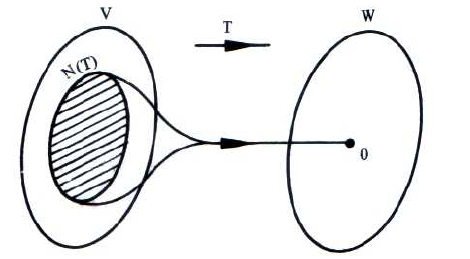
\includegraphics[scale=1.00]{t_nucleo.png}
	\caption{Diagrama do núcleo de uma transformação linear \cite{steinbruch1987}.}
\end{figure}

\noindent então, $\mathbf{N}(\mathbf{T}) \subset \mathbf{V}$ e $\mathbf{N}(\mathbf{T}) \neq \emptyset$, pois $0 \in \mathbf{N}(\mathbf{T})$, se $\mathbf{T}(0) = 0$.

De acordo com \cite{lang2003}, que, enfatizou a importância do núcleo na compreensão da injetividade de uma transformação linear, ou seja, a capacidade de preservar a identidade dos vetores. O núcleo de uma transformação linear possui duas propriedades, que regem:

\begin{enumerate}
	\item O núcleo de uma transformação linear $\mathbf{T}: \mathbf{V} \longrightarrow \mathbf{W}$ é um subespaço vetorial de $\mathbf{V}$.
	\item Uma transformação linear $\mathbf{T}: \mathbf{V} \longrightarrow \mathbf{W}$ é injetora se, e somente se, $\mathbf{N}(\mathbf{T}) = \{0\}$.
\end{enumerate}

Se $\mathbf{v}_1$ e $\mathbf{v}_2$ pertencem ao núcleo $\mathbf{N}(\mathbf{T})$ e $k$ um número real qualquer. Então, $\mathbf{T}(\mathbf{v}_1) = 0$ e $\mathbf{T}(\mathbf{v}_2) = 0$. Logo:

\begin{equation}
\mathbf{T}(\mathbf{v}_1 + \mathbf{v}_2) = \mathbf{T}(\mathbf{v}_1) + \mathbf{T}(\mathbf{v}_2) = 0 + 0 = 0
\end{equation}

\noindent portanto, $\mathbf{v}_1 + \mathbf{v}_2 \in \mathbf{N}(\mathbf{T})$. 

\noindent\textbf{Exemplo 14:} Dado $\mathbf{T}: \mathbb{R}^2 \longrightarrow \mathbb{R} \mid (x, y) \rightarrow x + y$, o núcleo, que iremos chamar, neste caso, $\ker\mathbf{T}$ é $\ker\mathbf{T} = \{(x, y) \in \mathbb{R}^2; x + y = 0\}$, onde a reta $y = -x$ é $\ker\mathbf{T}$ e $\ker\mathbf{T} = \{(x, -x); x \in \mathbb{R}\} = \{x(1, -1); x \in \mathbb{R}\} = [(1, -1)]$. A imagem da transformação, ou seja, $Im\mathbf{T} = \mathbb{R}$, todavia, um vetor $\mathbf{w} \in \mathbb{R}, \mathbf{w} = \mathbf{T}(\mathbf{w}, 0)$.

\begin{figure}[H]
	\centering
	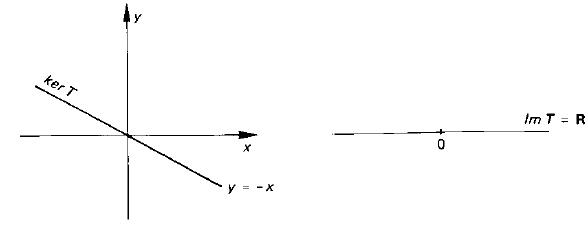
\includegraphics[scale=1.00]{t_nucleo2.png}
	\caption{Imagem de um núcleo de transformação linear \cite{boldrini1980}, pg. 152.}
\end{figure}

Percebe-se que a imagem de uma transformação é $\mathbf{T}: \mathbf{V} \longrightarrow \mathbf{W}$ é um subespaço de $\mathbf{W}$, pois, se tomarmos dois vetores, $\mathbf{w}_1 + \mathbf{w}_2 \in Im\mathbf{T}$ e $\alpha\mathbf{w}_1 \in Im\mathbf{T}$. Existem vetores $\mathbf{v}$ e $\mathbf{u} \in \mathbf{V} \mid \mathbf{T}(\mathbf{v}) = \mathbf{w}_1 + \mathbf{w}_2$ e $\mathbf{T}(\mathbf{u}) = \alpha\mathbf{w}_1$.

Se $\mathbf{w}_1, \mathbf{w}_2 \in Im\mathbf{T}$, existem vetores $\mathbf{v}_1, \mathbf{v}_2 \in \mathbf{V} \mid \mathbf{T}(\mathbf{v}_1) = \mathbf{w}_1$ e $\mathbf{T}(\mathbf{v}_2) = \mathbf{w}_2$. Tendo $\mathbf{v} = \mathbf{v}_1 + \mathbf{v}_2$ e $\mathbf{u} = \alpha\mathbf{v}_1$, logo:

\begin{equation}
\mathbf{T}(\mathbf{v}) = \mathbf{T}(\mathbf{v}_1 + \mathbf{v}_2) = \mathbf{T}(\mathbf{v}_1) + \mathbf{T}(\mathbf{v}_2) = \mathbf{w}_1 + \mathbf{w}_2
\end{equation}

\noindent e $\mathbf{T}(\mathbf{u}) = \mathbf{T}(\alpha\mathbf{v}_1) = \alpha\mathbf{T}(\mathbf{v}_1) = \alpha\mathbf{w}_1$, portanto, $Im\mathbf{T}$ é um subespaço vetorial de $\mathbf{W}$.

\section{Isomorfismo}
Um conceito intrigante surge com o isomorfismo. Uma transformação linear $\mathbf{T}: \mathbf{U} \longrightarrow \mathbf{V}$, entre espaços vetoriais $\mathbf{U}$ e $\mathbf{V}$, que é bijetora. Um isomorfismo só é válido se atender a duas condições cruciais:

\begin{enumerate}
	\item \textbf{Injetividade:} $\mathbf{T}$ é injetora, o que significa que mapeia vetores distintos do domínio para vetores distintos no contradomínio. Em outras palavras, $\mathbf{T}$ preserva a identidade.
	\item \textbf{Sobrejetividade:} $\mathbf{T}$ é sobrejetora, mapeando todo vetor em $\mathbf{V}$ a partir de um vetor em $\mathbf{U}$. Isso significa que a imagem de $\mathbf{T}$ abrange todo o espaço $\mathbf{V}$.
\end{enumerate}

\begin{figure}[H]
	\centering
	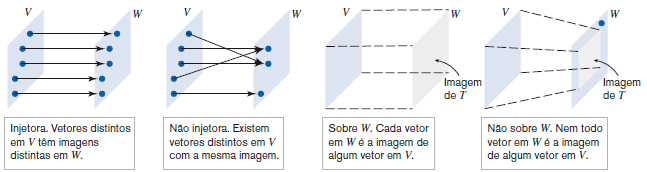
\includegraphics[scale=0.90]{t_isomorfismo.png}
	\caption{Diagrama do isomorfismo e sua imagem \cite{anton2010elementary}, pg. 445.}
\end{figure}

Se $\mathbf{T}$ satisfaz ambas as condições, podemos afirmar que ela estabelece uma correspondência biunívoca entre $\mathbf{U}$ e $\mathbf{V}$. Essa relação especial permite que representamos cada vetor em $\mathbf{V}$  por um único vetor em $\mathbf{U}$, e vice-versa. É notável também ressaltar, que, todo espaço vetorial $\mathbf{V}$ de dimensão $n$ é isomorfo a $\mathbb{R}^n$, portanto dois espaços vetoriais de dimensão finita são isomorfos se tiverem a mesma dimensão.

O núcleo de uma transformação e seu isomorfismo tem uma conexão que é o Teorema do Núcleo e da Imagem. Este teorema estabelece uma relação crucial entre a dimensão do núcleo, a dimensão da imagem e a dimensão do domínio de uma transformação linear $\mathbf{T}$:

\centerline{$\dim(\mathbf{N}(\mathbf{T})) + \dim(Im(\mathbf{T})) = \dim(\mathbf{U})$}

\noindent onde $Im(\mathbf{T})$ representa a imagem de $Im(\mathbf{T})$, o conjunto de todos os vetores em $\mathbf{V}$ que são alcançados por $\mathbf{T}$.

O Teorema do Núcleo e da Imagem oferece ferramentas valiosas para determinar se uma transformação linear é um isomorfismo. Se a dimensão do núcleo for zero e a dimensão da imagem for igual à dimensão do domínio, podemos concluir que $\mathbf{T}$ é um isomorfismo.

\noindent\textbf{Teorema 10:} Sejam $E, F$ espaços vetoriais de dimensão finita. Para toda transformação linear $\mathbf{T}: E \longrightarrow F$ tem-se que $\dim E = \dim \mathbf{N}(\mathbf{T}) + \dim Im(\mathbf{T})$.

Se $\{\mathbf{T}(\mathbf{u}_1), \ldots, \mathbf{T}(\mathbf{u}_p)\}$ é uma base de $Im(\mathbf{T})$ e $\{\mathbf{v}_1, \ldots, \mathbf{v}_q\}$ é uma base de $\mathbf{N}(\mathbf{T})$ então $\{\mathbf{u}_1, \ldots, \mathbf{u}_p, \mathbf{v}_1, \ldots, \mathbf{v}_q\}$ é uma base de $E$. Logo, se tivemos

\centerline{$\alpha_1\mathbf{u}_1 + \ldots + \alpha_p + \beta\mathbf{v}_1 + \ldots + \beta\mathbf{u}_q = 0$,}

então, com a transformação em ambos os membros da igualdade, obtemos

\centerline{$\alpha_1\mathbf{T}(\mathbf{u}_1) + \ldots + \alpha_p\mathbf{T}(\mathbf{u}_p) = 0$.}

Como $\mathbf{T}(\mathbf{u}_1), \ldots, \mathbf{T}(\mathbf{u}_p)$ são \textbf{LI}, resultando em $\alpha_1 = \ldots = \alpha_p = 0$. Portanto se reduz a igualdade

\centerline{$\beta_1\mathbf{v}_1 + \ldots + \beta_q\mathbf{v}_q = 0$.}

Da mesma forma $\mathbf{v}_1, \ldots, \mathbf{v}_q$ são \textbf{LI}, concluí-se que $\beta_1 = \ldots = \beta_q = 0$. Então ambos os vetores $\mathbf{u}$ e $\mathbf{v}$ são \textbf{LI}.

Agora, se considerarmos um vetor arbitrário $\mathbf{w} \in E$. Como $\mathbf{T}(\mathbf{w}) \in Im(\mathbf{T})$, definimos

\centerline{$\mathbf{T}(\mathbf{w}) = \alpha_1\mathbf{T}(\mathbf{u}_1) + \ldots + \alpha_p\mathbf{T}(\mathbf{u}_p)$,}

pois $\{\mathbf{T}(\mathbf{u}_1), \ldots, \mathbf{T}(\mathbf{u}_p)\}$ é uma base da imagem de $\mathbf{T}$. Manipulando a expressão temos

\centerline{$\mathbf{T}[\mathbf{w} - (\alpha_1\mathbf{u}_1 + \ldots + \alpha_p\mathbf{u}_p)] = 0$.}

Dessa forma, o vetor $\mathbf{w} - (\alpha_1\mathbf{u}_1 + \ldots + \alpha_p\mathbf{u}_p)$ pertence ao núcleo de $\mathbf{T}$, podendo ser expresso como uma combinação linear dos elementos da base $\{\mathbf{v}_1, \ldots, \mathbf{v}_q\}$. Temos então

\centerline{$(\alpha_1\mathbf{u}_1 + \ldots + \alpha_p\mathbf{u}_p) = \beta_1\mathbf{v}_1 + \ldots + \beta_q\mathbf{v}_q$,}

ou seja, $\mathbf{w} = \alpha_1\mathbf{u}_1 + \ldots + \alpha_p\mathbf{u}_p + \beta_1\mathbf{v}_1 + \ldots + \beta_q\mathbf{v}_q$. O que prova que os vetores $\{\mathbf{u}_1, \ldots, \mathbf{u}_p, \mathbf{v}_1, \ldots, \mathbf{v}_q\}$ geram $E$ e portanto constituem uma base.
